\begin{figure}[ht!]
    \begin{center}
        % This file was created by matlab2tikz.
%
%The latest updates can be retrieved from
%  http://www.mathworks.com/matlabcentral/fileexchange/22022-matlab2tikz-matlab2tikz
%where you can also make suggestions and rate matlab2tikz.
%
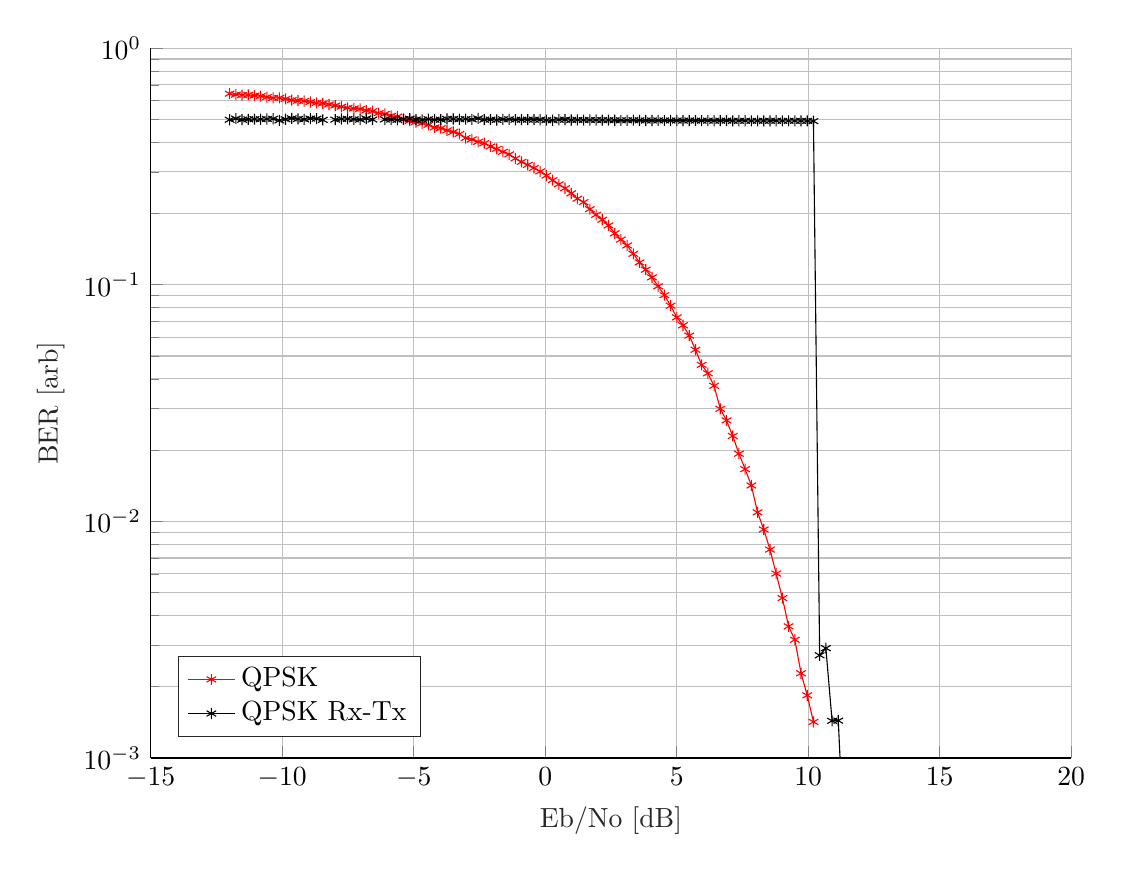
\begin{tikzpicture}

\begin{axis}[%
width=4.602in,
height=3.549in,
at={(0.772in,0.479in)},
scale only axis,
unbounded coords=jump,
xmin=-15,
xmax=20,
xlabel style={font=\color{white!15!black}},
xlabel={Eb/No [dB]},
ymode=log,
ymin=0.001,
ymax=1,
yminorticks=true,
ylabel style={font=\color{white!15!black}},
ylabel={BER [arb]},
axis background/.style={fill=white},
axis x line*=bottom,
axis y line*=left,
xmajorgrids,
ymajorgrids,
yminorgrids,
legend style={at={(0.03,0.03)}, anchor=south west, legend cell align=left, align=left, draw=white!15!black}
]
\addplot [color=red, mark=asterisk, mark options={solid, red}]
  table[row sep=crcr]{%
-12	0.642227155456892\\
-11.7638190954774	0.636387272254555\\
-11.5276381909548	0.633667326653467\\
-11.2914572864322	0.634447311053779\\
-11.0552763819095	0.630627387452251\\
-10.8190954773869	0.627047459050819\\
-10.5829145728643	0.621227575448491\\
-10.3467336683417	0.616127677446451\\
-10.1105527638191	0.616187676246475\\
-9.87437185929648	0.610127797444051\\
-9.63819095477387	0.603307933841324\\
-9.40201005025126	0.599968000639987\\
-9.16582914572864	0.59782804343913\\
-8.92964824120603	0.59232815343693\\
-8.69346733668342	0.587368252634947\\
-8.4572864321608	0.584528309433811\\
-8.22110552763819	0.577968440631187\\
-7.98492462311558	0.572348553028938\\
-7.74874371859297	0.565508689826203\\
-7.51256281407035	0.559588808223836\\
-7.27638190954774	0.55614887702246\\
-7.04020100502513	0.55334893302134\\
-6.80402010050251	0.545069098618028\\
-6.5678391959799	0.541629167416652\\
-6.33165829145729	0.531709365812684\\
-6.09547738693467	0.52734945301094\\
-5.85929648241206	0.517429651406972\\
-5.62311557788945	0.513709725805485\\
-5.38693467336683	0.500089998200036\\
-5.15075376884422	0.493810123797525\\
-4.91457286432161	0.487510249795004\\
-4.678391959799	0.481370372592549\\
-4.44221105527638	0.474130517389652\\
-4.20603015075377	0.462470750584988\\
-3.96984924623116	0.458990820183596\\
-3.73366834170854	0.449191016179676\\
-3.49748743718593	0.442631147377052\\
-3.26130653266332	0.433891322173557\\
-3.0251256281407	0.416971660566788\\
-2.78894472361809	0.411431771364572\\
-2.55276381909548	0.401951960960781\\
-2.31658291457286	0.396692066158676\\
-2.08040201005025	0.384272314553709\\
-1.84422110552764	0.375032499350013\\
-1.60804020100502	0.364812703745924\\
-1.37185929648241	0.355672886542269\\
-1.1356783919598	0.341913161736765\\
-0.899497487437186	0.33077338453231\\
-0.663316582914574	0.321173576528469\\
-0.427135678391959	0.31167376652467\\
-0.190954773869347	0.301313973720526\\
0.0452261306532655	0.28947421051579\\
0.28140703517588	0.276654466910662\\
0.517587939698492	0.26577468450631\\
0.753768844221106	0.25577488450231\\
0.989949748743719	0.24347513049739\\
1.22613065326633	0.231095378092438\\
1.46231155778895	0.223515529689406\\
1.69849246231156	0.208735825283495\\
1.93467336683417	0.197616047679047\\
2.17085427135678	0.188336233275334\\
2.4070351758794	0.17817643647127\\
2.64321608040201	0.164976700465991\\
2.87939698492462	0.155316893662127\\
3.11557788944724	0.146597068058639\\
3.35175879396985	0.135097298054039\\
3.58793969849246	0.124337513249735\\
3.82412060301507	0.115797684046319\\
4.06030150753769	0.107457850842983\\
4.2964824120603	0.0985380292394151\\
4.53266331658292	0.0903781924361511\\
4.76884422110553	0.0815583688326234\\
5.00502512562814	0.0728185436291274\\
5.24120603015075	0.0674186516269674\\
5.47738693467337	0.0609787804243916\\
5.71356783919598	0.0531189376212475\\
5.94974874371859	0.0458590828183436\\
6.18592964824121	0.0422591548169037\\
6.42211055276382	0.0374192516149677\\
6.65829145728643	0.0298994020119597\\
6.89447236180904	0.0267194656106878\\
7.13065326633166	0.0229595408091838\\
7.36683417085427	0.0193196136077278\\
7.60301507537688	0.0166196676066478\\
7.8391959798995	0.0141797164056719\\
8.07537688442211	0.0109197816043679\\
8.31155778894473	0.00923981520369593\\
8.54773869346734	0.00759984800303993\\
8.78391959798995	0.00601987960240795\\
9.02010050251256	0.00473990520189596\\
9.25628140703517	0.00359992800143997\\
9.49246231155779	0.00315993680126397\\
9.7286432160804	0.00227995440091198\\
9.96482412060302	0.00183996320073598\\
10.2010050251256	0.00141997160056799\\
};
\addlegendentry{QPSK}

\addplot [color=black, mark=asterisk, mark options={solid, black}]
  table[row sep=crcr]{%
-12	0.498225108225109\\
-11.7638190954774	0.503930280246069\\
-11.5276381909548	0.498515769944342\\
-11.2914572864322	0.500494743351887\\
-11.0552763819095	0.501396103896104\\
-10.8190954773869	0.500699300699301\\
-10.5829145728643	0.501974025974026\\
-10.3467336683417	0.503019480519481\\
-10.1105527638191	0.495075757575757\\
-9.87437185929648	0.500529100529101\\
-9.63819095477387	0.505194805194805\\
-9.40201005025126	0.502095631641086\\
-9.16582914572864	0.500077922077923\\
-8.92964824120603	0.50416951469583\\
-8.69346733668342	0.503339517625232\\
-8.4572864321608	0.497591991341991\\
nan	nan\\
-7.98492462311558	0.499047619047618\\
-7.74874371859297	0.501898101898103\\
-7.51256281407035	0.502481447124304\\
-7.27638190954774	0.500628403854211\\
-7.04020100502513	0.498944805194805\\
-6.80402010050251	0.504347826086956\\
-6.5678391959799	0.499413489736071\\
nan	nan\\
-6.09547738693467	0.499533799533799\\
-5.85929648241206	0.499055489964581\\
-5.62311557788945	0.49759111855886\\
-5.38693467336683	0.500987012987013\\
-5.15075376884422	0.5036866359447\\
-4.91457286432161	0.4991926991927\\
-4.678391959799	0.498011363636363\\
-4.44221105527638	0.501233766233766\\
-4.20603015075377	0.498293135435992\\
-3.96984924623116	0.498484848484849\\
-3.73366834170854	0.502431289640591\\
-3.49748743718593	0.502050580997949\\
-3.26130653266332	0.500553857906798\\
-3.0251256281407	0.501654298082869\\
-2.78894472361809	0.499942279942279\\
-2.55276381909548	0.50456400742115\\
-2.31658291457286	0.498749398749398\\
-2.08040201005025	0.49911754911755\\
-1.84422110552764	0.497066326530612\\
-1.60804020100502	0.500304383116883\\
-1.37185929648241	0.500413223140497\\
-1.1356783919598	0.49825487012987\\
-0.899497487437186	0.498411723411724\\
-0.663316582914574	0.498697386950399\\
-0.427135678391959	0.498483424470266\\
-0.190954773869347	0.498335467349552\\
0.0452261306532655	0.496386483886483\\
0.28140703517588	0.495711648757334\\
0.517587939698492	0.498267459221906\\
0.753768844221106	0.498456213047654\\
0.989949748743719	0.496865203761755\\
1.22613065326633	0.497449226305608\\
1.46231155778895	0.496835460676662\\
1.69849246231156	0.497144787272176\\
1.93467336683417	0.496925498165956\\
2.17085427135678	0.496642758382302\\
2.4070351758794	0.496500721500722\\
2.64321608040201	0.495818815331011\\
2.87939698492462	0.495596661124343\\
3.11557788944724	0.495471114547663\\
3.35175879396985	0.496093870500047\\
3.58793969849246	0.49563909774436\\
3.82412060301507	0.494533686837181\\
4.06030150753769	0.494713305562362\\
4.2964824120603	0.494958767468273\\
4.53266331658292	0.494844499064448\\
4.76884422110553	0.494690860950339\\
5.00502512562814	0.49452894563064\\
5.24120603015075	0.494082332761579\\
5.47738693467337	0.494666644409575\\
5.71356783919598	0.49408103592314\\
5.94974874371859	0.493831168831169\\
6.18592964824121	0.49429967799533\\
6.42211055276382	0.493406804463142\\
6.65829145728643	0.49369629738948\\
6.89447236180904	0.494238166205378\\
7.13065326633166	0.492853727469111\\
7.36683417085427	0.493271364204308\\
7.60301507537688	0.493273869744457\\
7.8391959798995	0.492731372426396\\
8.07537688442211	0.493171136957038\\
8.31155778894473	0.493084166791063\\
8.54773869346734	0.493158268965476\\
8.78391959798995	0.493250736605166\\
9.02010050251256	0.492728315614475\\
9.25628140703517	0.492924478587238\\
9.49246231155779	0.492771297483223\\
9.7286432160804	0.492891614212287\\
9.96482412060302	0.492634013192813\\
10.2010050251256	0.491615839757104\\
10.4371859296482	0.00271639389433625\\
10.6733668341709	0.00291077243748846\\
10.9095477386935	0.00143514351435144\\
11.1457286432161	0.00143780611827416\\
11.3374209303722	0.000501187233627271\\
};
\addlegendentry{QPSK Rx-Tx}

\end{axis}
\end{tikzpicture}%
        \caption{Comparison of BER results }
    \end{center}\label{fig:4}
\end{figure}

Figure~\ref{fig:4} shows Eb/N0 vs BER for a QPSK signal in the presence of AWGN noise, vs a QPSK rx/tx communication link simulating additional: time delay, frequency offset distortions and filers present in typical communication links. The results are obtained using the Matlab script as shown in \ref{matlabs:task4}. The graph shows the simulated comms link is almost a perfect step whereases the simple model shows the BER decreasing smoothly as the signal strength increases. In the real world, this would make the comms link very binary, either having a connection or not. 

For the comms link, the additional distortions further scramble the signal. The filters in the comms link can rebuild the signal in the presence of AWGN noise by comparing what they see to what they expect to see. However, if the noise is large enough these filters can't synchronize, and the signal becomes scrabbled. In practice, these links are either connected or not.